%anatomy
\section{Anatomy of the human lower forearm} \label{sec:anatomy}
%\section{Anatomy of the distal part of the arm} \label{sec:anatomy} 		%%old

%arguments for choice of movements (header)
%anatomy/physiology of arm and muscles
%segue to EMG

%head
This project will use six movements for control of a virtual interface and visual feedback. The movements are extension, flexion, radial and ulnar deviation, closed and opened hand as well as rest. The movements are shown in \figref{fig:handMovements}. %These six movements cover DOFs which will be used in the control scheme for testing performance in a virtual target reaching test, described in \secref{sec:fitts}. 
These movements are either individually or in combination most often used during many daily life tasks. Thus training users to improve performance of these movements for use in a myoelectric prosthesis control scheme, would prove to cover most functions a prosthesis should cover for use in daily life tasks. 

%In this project recordings of EMG signals will be used for control and test of the effect of providing class certainty feedback during user training. The recordings will be made with a Myo armband (MYB) described in \secref{sec:MYB}. The recordings will be recorded from the lower forearm of test subjects on muscles involved with performing the six different stated movements. 

\begin{figure}[H] 
	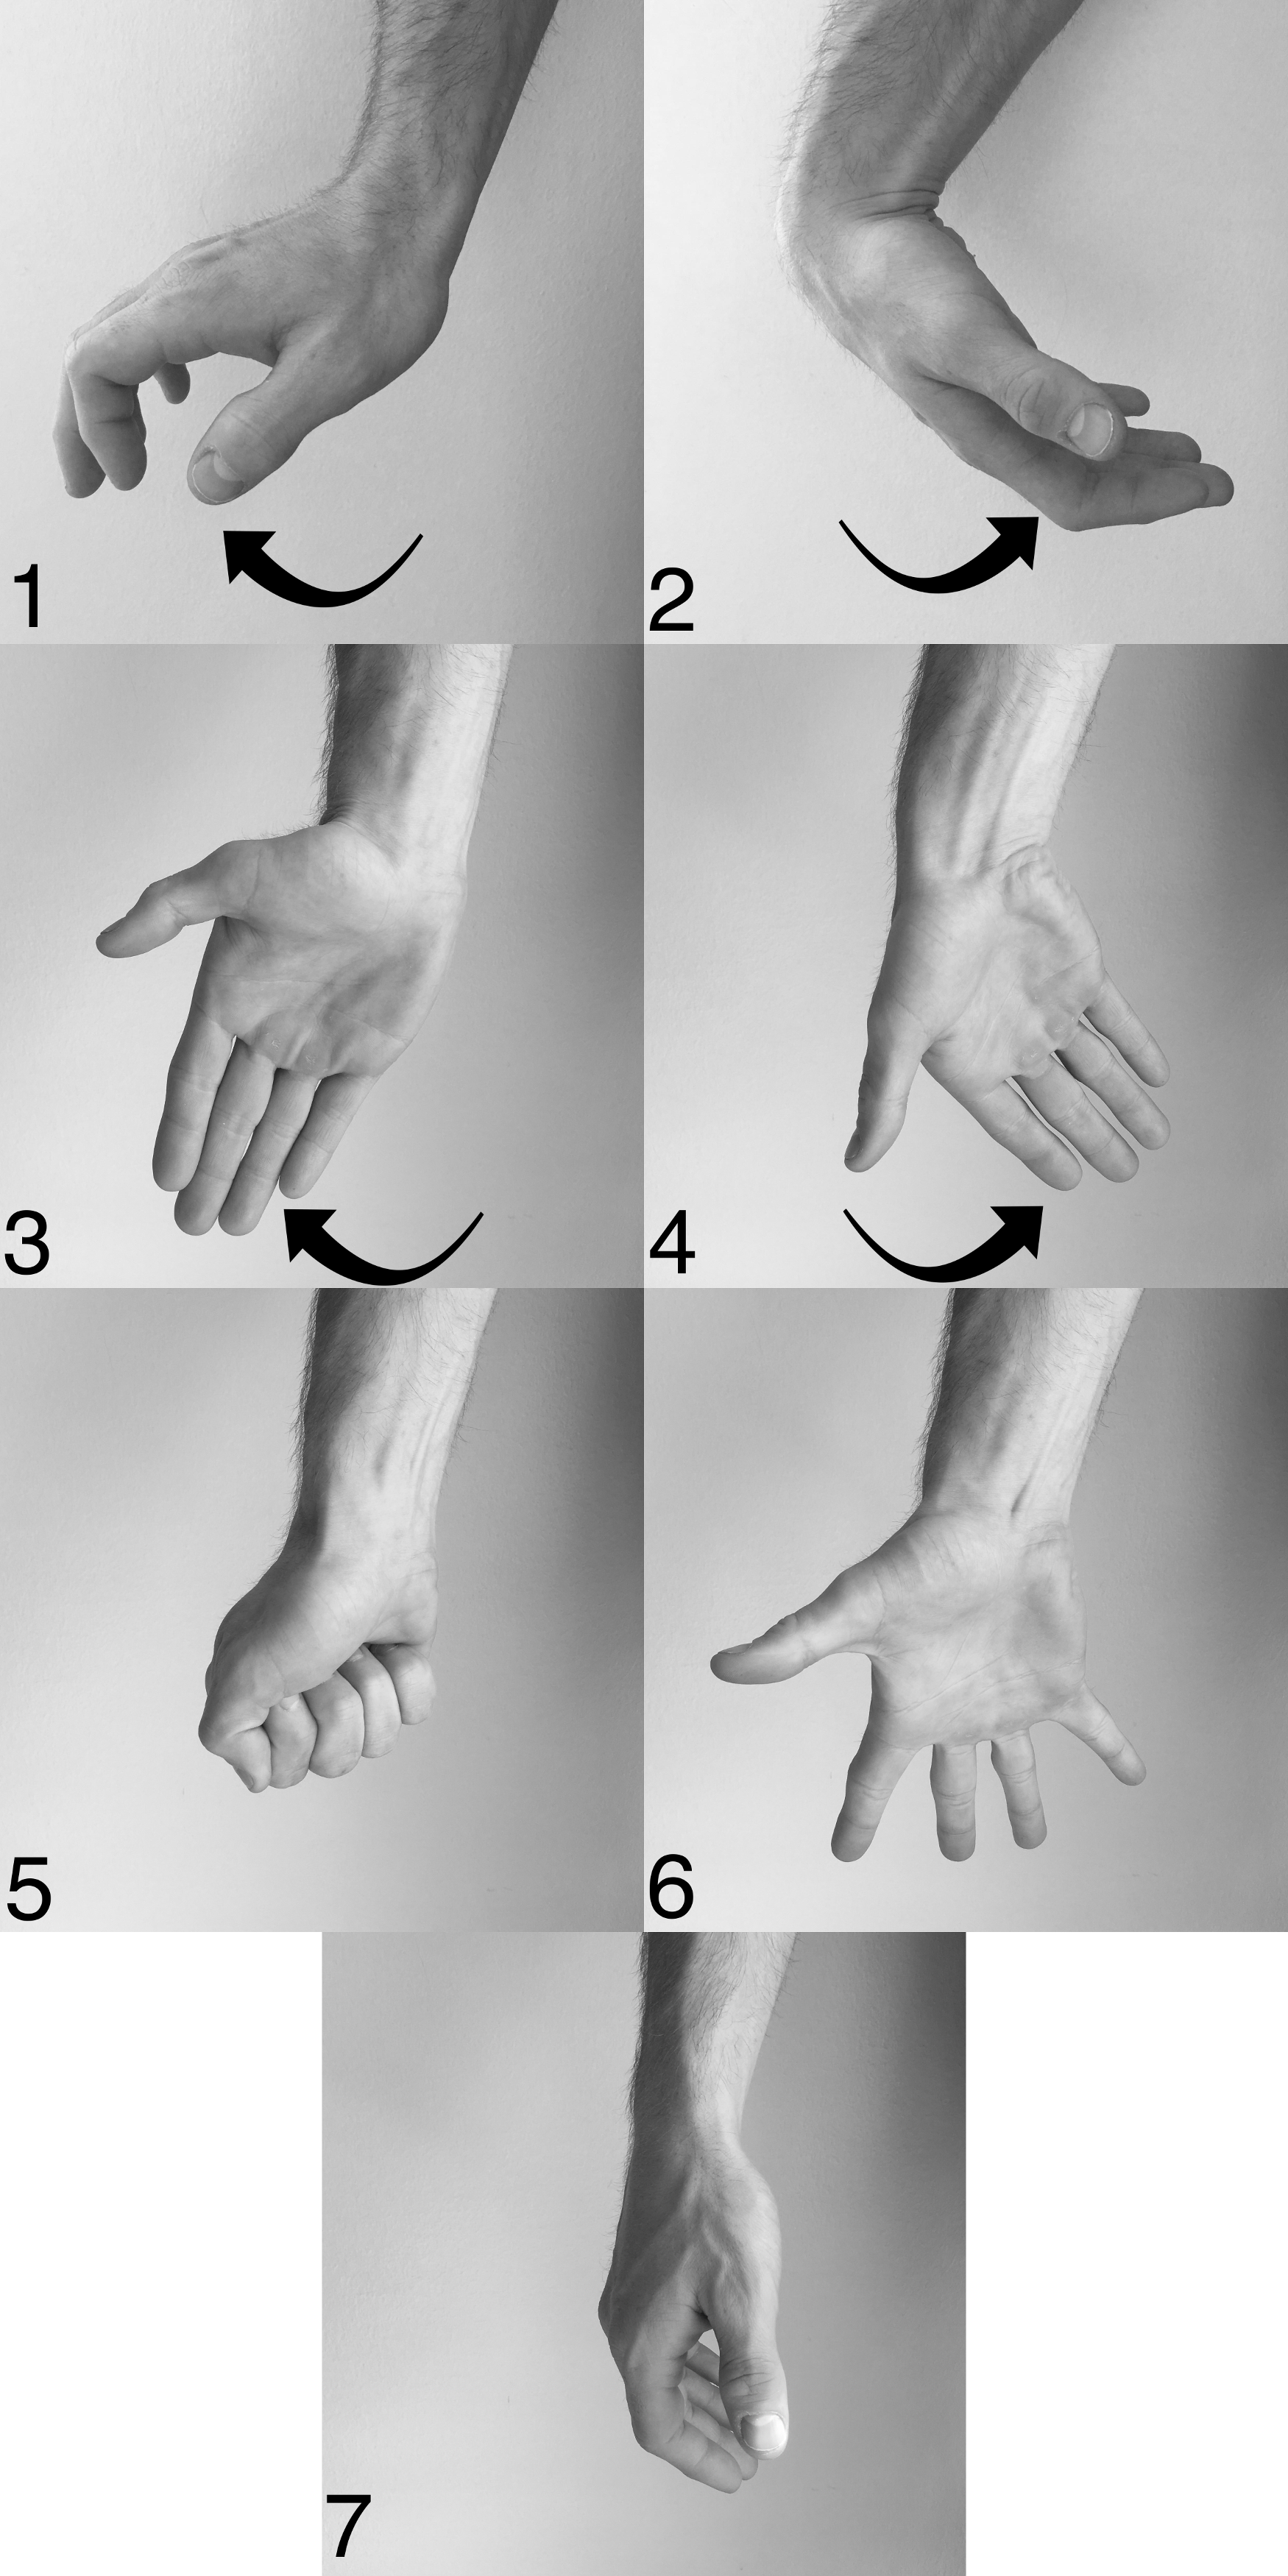
\includegraphics[width=0.4\textwidth]{figures/handGestures/BW/allHandMovementsVerticalBW}
	\caption{The figure shows the six hand movements used in this study as well as rest. The movements are: 1) extension, 2) flexion, 3) radial deviation, 4) ulnar deviation, 5) closed hand, 6) opened hand and 7) rest.}
	\label{fig:handMovements}
\end{figure}

The human arm has five DOFs being covered by the movements extension, flexion, abduction, adduction and rotation at the shoulder, flexion at the elbow and supination and pronation of the lower forearm. 
%Three of the five DOFs covered by movements at the shoulder is illustrated in \figref{fig:armMovements}.

%\begin{figure}[H] 
%	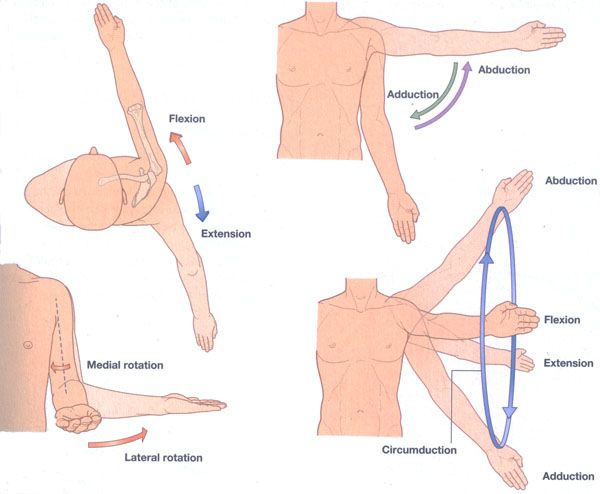
\includegraphics[width=0.5\textwidth]{figures/xBackground/aAnatomy/armMovements}
%	\caption{Movements at the shoulder: extension, flexion, abduction, adduction and rotation in medial and lateral direction. The movements cover three of the five DOFs of the arm. \cite{Kim2015}}
%	\label{fig:armMovements}
%\end{figure}

The human hand is a very versatile and dexterous apparatus possessing a total of 25 active DOFs. These DOFs are expressed at the fingers, wrist and palm, where the fingers account for a total of 21 DOFs and the wrist account for two DOFs. Each finger posses four DOFs, while the thumb has five, also being able to do opposition movement to each other finger. At the wrist the hand can flex and extend as well as perform radial and ulnar deviations. The last two DOFs exist in the palm of the hand where the joints between the fourth and fifth metacarpal bones and the hamate bone of the carpal bones in the wrist give the hand movement along two additional axes which is used when doing opposition of the thumb and the fifth finger. \cite{Martini2012}

Many of these DOFs and corresponding movements are active when using the hand. The chosen movements for this project will involve most of the DOFs in the hand, as can be seen on \figref{fig:handMovements}. Movements at the wrist (extension/flexion, radial/ulnar deviation) are DOFs of the hand. Even though many individual movements of joints and DOFs of the hand and fingers are active during opening and closing of the hand. During the rest of the project these two movements will be described as being movement in one DOF. 

\subsection{Muscles of the lower forearm}

To perform movements of the hand and fingers and at the wrist, muscles in the lower arm are active. All movements relevant for this study are controlled by muscles in the lower forearm, thus it is relevant to gain knowledge on the muscles in the lower forearm. When performing actions at the wrist the following muscles are active: flexor carpi radialis, flexor carpi ulnaris, palmaris longus, extensor carpi radialis longus, extensor carpi radialis brevis, extensor carpi ulnaris. The flexor and extensor muscles are naturally responsible for performing flexion and extension respectively at the wrist. They are however also responsible for performing radial and ulnar deviation, where the flexor carpi radialis and extensor carpi radialis brevis muscles, which are antoganistic muscles when doing flexion and extension, will work together when performing radial deviation. The extensor carpi radialis longus muscle is also responsible for performing radial deviation. The flexor and extensor carpi ulnaris muscles are responsible when performing ulnar deviation. The palmaris longus muscle is only active during flexion at the wrist. \cite{Martini2012}

Several more muscles are further specified to perform movements of the fingers but many of these are also active during extension/flexion and radial/ulnar deviations at the wrist. Muscles responsible when opening the hand by extending the fingers are: extensor digitorum, extensor pollicis brevis, extensor pollicis longus, extensor indicis and the extensor digiti minimi muscle. Contrary, the muscles responsible for closing the hand by flexing the fingers are: flexor digitorum superficialis, flexor digitorum profundus and the flextor pollicis longus. \cite{Martini2012}







%being able to perform extension, flexion at both its joint between the distal/proximal phalanges and proximal phlanges and metacarpal bone. It can perform abducation, adducation, fl
%
%
%%EMG recordings will be measured from the distal forearm of test subjects, in order to use EMG signals for control and test the effect of providing feedback during user training. Recordings will be recorded with a Myo armband (MYB) from Thalmic Labs, further described in \secref{sec:MYB}. This section will provide information on the anatomy of the distal part of the arm and the general muscles involved in movements used in this project.\\
%
%
%The human arm is the base and extender for our greatest tool: the hand. The human hand is a very versatile and dexterous tool, and the loss of that function is therefore a great loss in relation to functionality and independence. The hand gains its vast utilization by having 27 degrees of freedom (DOF). This in itself makes it very dexterous but it is the arm that moves the hand along seven DOFs, that enables the hand to use its dexterity.\\
%Movement of limbs are caused by muscle contractions. The muscles contract when receiving nerve impulses from the central nervous system (CNS). \cite{Martini2012} \\
%The greater workings of muscle activation is described further in \secref{sec:EMG}.  
%Many muscles in the lower forearm are involved when performing hand gestures. Several muscles are actors in performing specific movements, and some of these are at times antagonistic muscles but will work together when performing other movements. The flexor carpi radialis and extensor carpi radialis brevis muscles are as an example antagonists in performing flexion and extension at the wrist, but are both involved when doing abduction of the wrist. \cite{Martini2012} 
%NO -- This can prove a problem when recording EMG signals from these muscles, since if based only on the recording there is no way of knowing which muscle and under which movement the signal is recorded from. However, this problem is overcome when doing EMG recordings of several muscles at the same time. As with the MYB, recordings are made in a circle all the way around one section of the forearm, providing a recording of several muscles at the same time. This enables a control system to evaluate individual muscle recordings in relation the recordings of other muscles, thus making correct classification of different hand gestures possible. \cite{Mendez2017}
%
%
%
%
%
%%Looking closer at the anatomy and arrangement of the muscles involved in performing these four movements, several of the muscles are active during movements in both DOFs. As noted on \figref{fig:lowerArm} a total of five muscles in the distal part of the forearm are activated during both flexion/extension and ulnar/radial deviation at the wrist. However, according to \cite{Mendez2017} et al. the MYB has no problem correctly classifying different hand gestures, even when the active muscles are anatomically overlapping. %maybe more 
%%
%%\begin{figure}[H]
%%	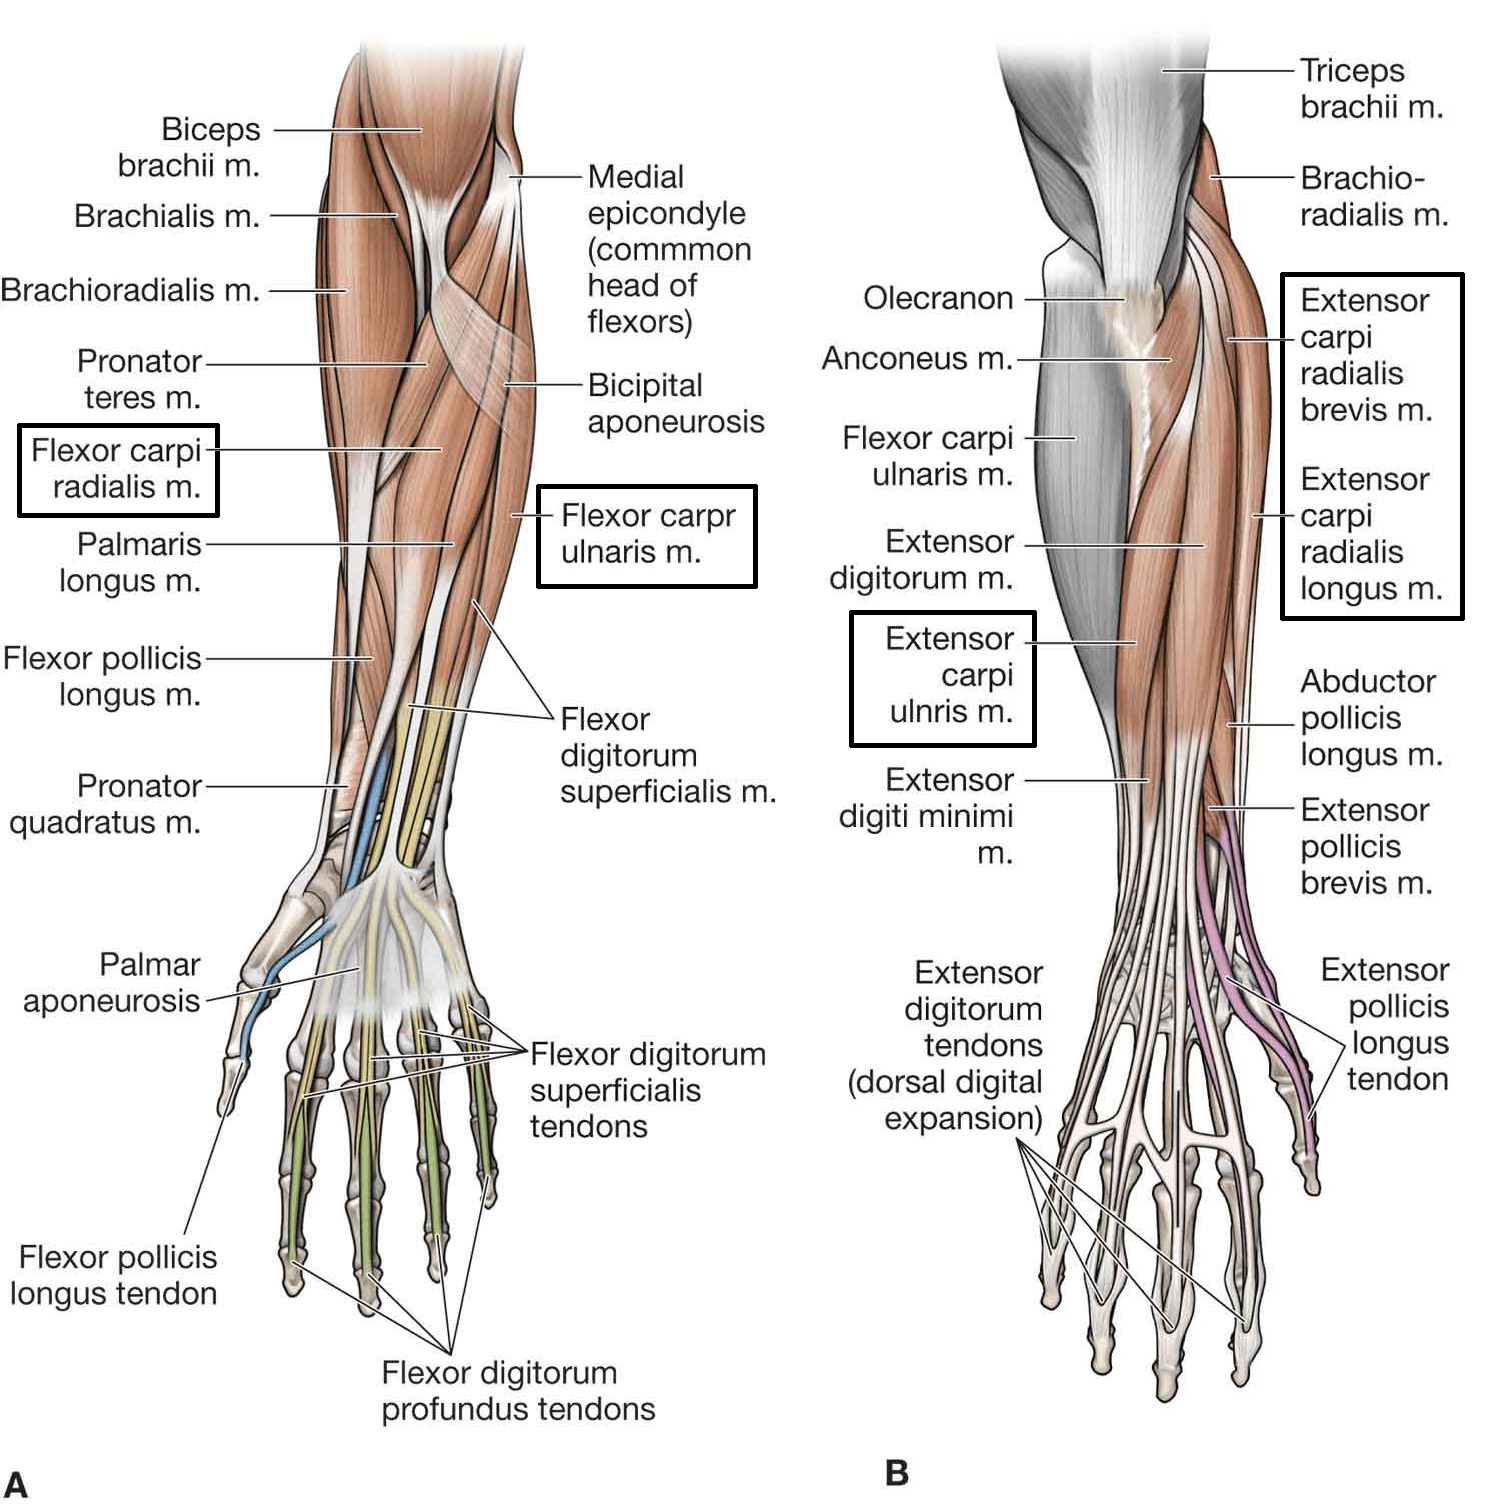
\includegraphics[width=0.7\textwidth]{figures/xBackground/aAnatomy/lowerArm}
%%	\caption{\textbf{A)} anterior view of lower muscles. \textbf{B)} posterior view of lower muscles. The boxed names are of muscles included in both flexion/extension and ulnar/radial deviation. \cite{7semesterprojekt}}
%%	\label{fig:lowerArm}
%%\end{figure}
%
%
%
%
